\begin{frame}{Το έργο RELIEF: motivation}



\noindent\makebox[\linewidth][c]{%
\begin{minipage}{\linewidth}
 \hspace{0.5cm}
 \begin{minipage}{0.4\linewidth}
  Αποθήκες προϊόντων: ανάγκη για

  \begin{itemize}
    \item συνεχή απογραφή
    \item γνώση θέσης προϊόντων
  \end{itemize}
  \end{minipage}
  \hspace{0.5cm}
  \begin{minipage}{0.5\linewidth}
    \begin{figure}
      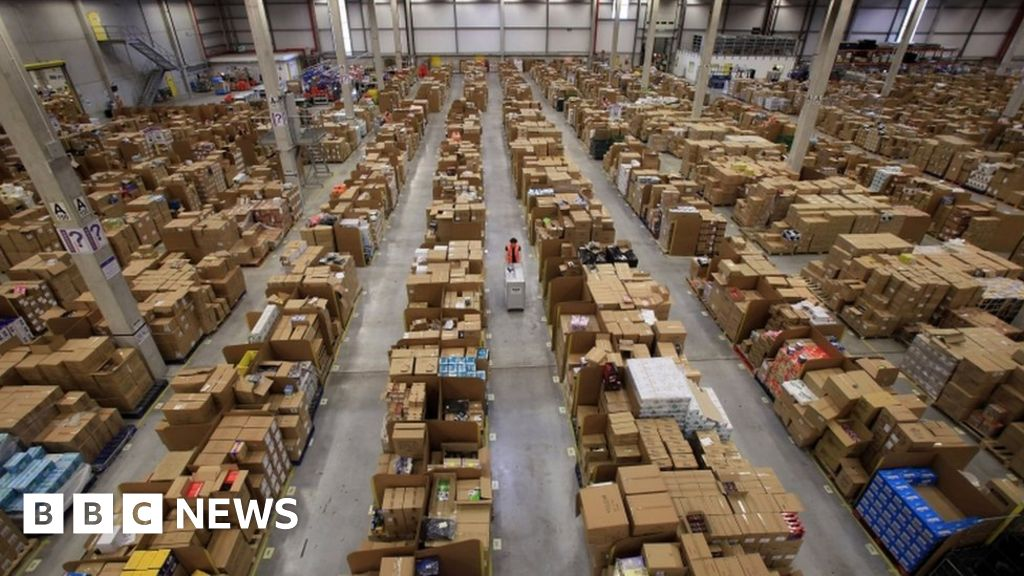
\includegraphics[height=101pt,width=180pt]{./figures/slides/01/relief_warehouse.jpg}
      \caption{\scriptsize Πηγή: BBC---\textit{Amazon sellers hit by 'extensive' fraud campaign}, \tiny \url{https://www.bbc.com/news/technology-48215073}}
    \end{figure}
  \end{minipage}
\end{minipage}
}

\note{\footnotesize
Τώρα---όλα αυτά που θα δούμε ξεκινάνε από μία πραγματική και εκτεταμένη
απάιτηση στην αγορά λιανικών προϊόντων. Εκεί υπάρχουν εταιρείες που πουλάνε τα
προϊόντα τους σε καταστήματα, και των οποίων το συνολικό απόθεμα αποθηκεύεται
σε κεντρικές αποθήκες. Εν γένει αυτές οι εταιρείες θα ήθελαν να γνωρίζουν σε
καθημερινή βάση το απόθεμά που βρίσκεται στις αποθήκες τους, όμως αυτό είναι
τόσο κοστοβόρο που μπορούν να μετρούν το απόθεμά τους μόνο λίγες φορές μέσα
σε ένα οικονομικό έτος. Έπειτα θα ήθελαν επίσης να γνωρίζουν τις θέσεις των
προϊόντων μέσα σε ένα κατάστημα ή μία αποθήκη τόσο για λόγους γρήγορης
ανάκτησης όσο και για λόγους που τους επιβάλλονται από τρίτα μέρη.}

\end{frame}
